\documentclass{article}

% content/resources/templates/preamble.tex
\usepackage[margin=0.6in]{geometry}
\author{Milav Dabgar}
\usepackage{amsmath,amssymb,amsthm}
\usepackage{booktabs}
\usepackage{multirow}
\usepackage{xcolor}
\usepackage{tcolorbox}
\tcbuselibrary{breakable,skins}
\usepackage[colorlinks=true,linkcolor=blue]{hyperref}
\usepackage{titlesec}
\usepackage{enumitem}
\usepackage{tikz}
\usepackage{pgfplots}
\usepackage{circuitikz}
\usepackage[version=4]{mhchem}
\usepackage{longtable}
\usepackage{array}
\usepackage{float}
\usepackage{caption}
\usepackage{listings}

\lstset{
  basicstyle=\small\ttfamily,
  breaklines=true,
  breakatwhitespace=false,
  postbreak=\mbox{\textcolor{red}{$\hookrightarrow$}\space},
  float=false,
  numbers=left,
  numberstyle=\tiny\color{gray},
  numbersep=10pt,
  xleftmargin=2em,
  keywordstyle=\color{blue},
  commentstyle=\color{green!60!black},
  stringstyle=\color{purple},
  backgroundcolor=\color{gray!5},
  showstringspaces=false,
  tabsize=2,
  captionpos=b,
  keepspaces=true,
  columns=flexible
}

\pgfplotsset{compat=1.18}
\usetikzlibrary{shapes,arrows,positioning,calc,patterns,decorations.pathmorphing,decorations.markings,arrows.meta}

% Color scheme
\definecolor{headcolor}{RGB}{0,102,204}
\definecolor{keycolor}{RGB}{220,20,60}
\definecolor{solutioncolor}{RGB}{34,139,34}
\definecolor{mnemoniccolor}{RGB}{148,0,211}
\definecolor{codecolor}{RGB}{0,0,100}

% Spacing
\setlength{\parskip}{3pt}
\setlist[itemize]{nosep}
\setlist[enumerate]{nosep}

% Title formatting
\titleformat{\section}{\Large\bfseries\color{headcolor}}{\thesection}{1em}{}
\titleformat{\subsection}{\large\bfseries\color{headcolor}}{\thesubsection}{1em}{}

% Pandoc tightlist compatibility
\providecommand{\tightlist}{%
  \setlength{\itemsep}{0pt}\setlength{\parskip}{0pt}}

% Pandoc longtable compatibility
\newcounter{none}
\def\thenone{}


% content/resources/templates/english-boxes.tex

% Custom environments
\newtcolorbox{solutionbox}{
 breakable,
 enhanced,
 colback=solutioncolor!5!white,
 colframe=solutioncolor!75!black,
 fonttitle=\bfseries,
 title=Solution
}

\newtcolorbox{solutionboxnobreak}{
 colback=solutioncolor!5!white,
 colframe=solutioncolor!75!black,
 fonttitle=\bfseries,
 title=Solution
}

\newtcolorbox{keyformula}{
 breakable,
 enhanced,
 colback=keycolor!5!white,
 colframe=keycolor!75!black,
 fonttitle=\bfseries,
 title=Key Formula
}

\newtcolorbox{mnemonicboxenv}{
 breakable,
 enhanced,
 colback=mnemoniccolor!5!white,
 colframe=mnemoniccolor!75!black,
 fonttitle=\bfseries,
 title=Mnemonic
}

\newcommand{\mnemonicbox}[1]{%
  \begin{mnemonicboxenv}
    #1
  \end{mnemonicboxenv}
}


% Custom commands for GTU solutions
% This file defines semantic commands for consistent formatting

% Question command with automatic formatting
\newcommand{\question}[2]{%
  \section*{Question #1}%
  \textbf{#2}%
}

% OR question variant
\newcommand{\questionor}[2]{%
  \section*{Question #1 OR}%
  \textbf{#2}%
}

% Proper table environment with caption
\newenvironment{answertable}[1]{%
  \begin{table}[htbp]
  \centering
  \caption{#1}
}{%
  \end{table}
}

% Proper figure environment for diagrams
\newenvironment{answerdiagram}[1]{%
  \begin{figure}[htbp]
  \centering
  \caption{#1}
}{%
  \end{figure}
}

% Semantic markup for key terms
\newcommand{\keyword}[1]{\textbf{#1}}
\newcommand{\code}[1]{\texttt{#1}}
\newcommand{\classname}[1]{\texttt{#1}}
\newcommand{\methodname}[1]{\texttt{#1}}

% Proper quotation marks
\newcommand{\mnemonic}[1]{``#1''}


\title{Microwave and Radar Communication (4351103) - Winter 2023 Solution}
\date{December 8, 2023}

\begin{document}
\maketitle

\questionmarks{1(a)}{3}{Sketch the standing wave pattern for voltage and current along the transmission line when it is terminated with (i) Short Circuit, (ii) Open circuit, and (iii) Matched Load.}

\begin{solutionbox}
\textbf{Standing Wave Patterns:}

\begin{answerdiagram}{Standing Wave Patterns}
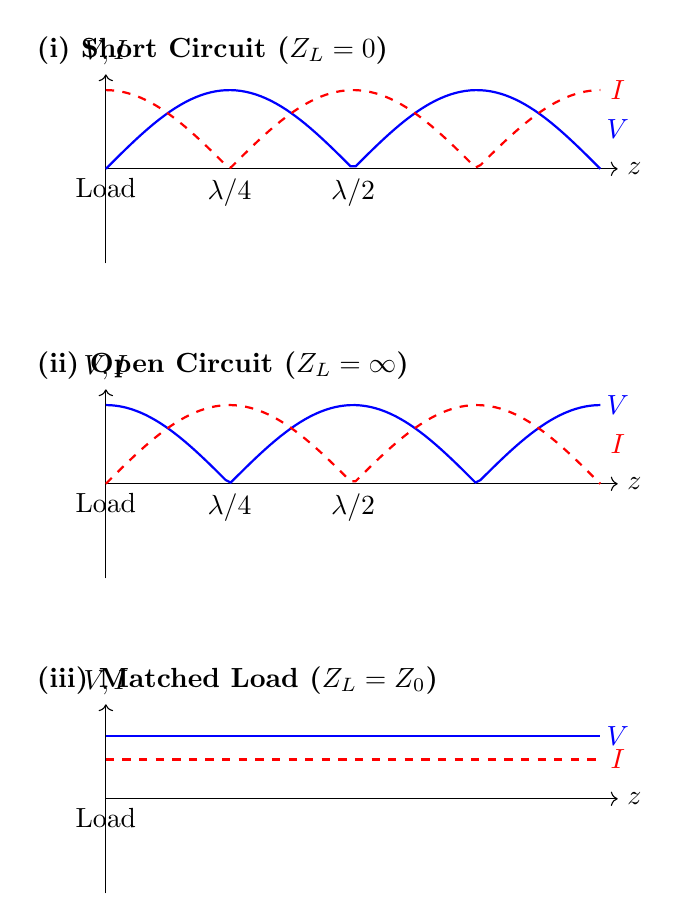
\begin{tikzpicture}
    % Short Circuit
    \begin{scope}[yshift=4cm]
        \node[anchor=west] at (-1, 1.5) {\textbf{(i) Short Circuit ($Z_L=0$)}};
        \draw[->] (0,0) -- (6.5,0) node[right] {$z$};
        \draw[->] (0,-1.2) -- (0,1.2) node[above] {$V, I$};
        
        \draw[blue, thick] plot[domain=0:6.28, samples=100, variable=\x] ({\x}, {abs(sin(\x*180/3.14))});
        \node[blue] at (6.5, 0.5) {$V$};
        
        \draw[red, thick, dashed] plot[domain=0:6.28, samples=100, variable=\x] ({\x}, {abs(cos(\x*180/3.14))});
        \node[red] at (6.5, 1) {$I$};
        
        \node[below] at (0,0) {Load};
        \node[below] at (1.57,0) {$\lambda/4$};
        \node[below] at (3.14,0) {$\lambda/2$};
    \end{scope}

    % Open Circuit
    \begin{scope}[yshift=0cm]
        \node[anchor=west] at (-1, 1.5) {\textbf{(ii) Open Circuit ($Z_L=\infty$)}};
        \draw[->] (0,0) -- (6.5,0) node[right] {$z$};
        \draw[->] (0,-1.2) -- (0,1.2) node[above] {$V, I$};
        
        \draw[blue, thick] plot[domain=0:6.28, samples=100, variable=\x] ({\x}, {abs(cos(\x*180/3.14))});
        \node[blue] at (6.5, 1) {$V$};
        
        \draw[red, thick, dashed] plot[domain=0:6.28, samples=100, variable=\x] ({\x}, {abs(sin(\x*180/3.14))});
        \node[red] at (6.5, 0.5) {$I$};
        
        \node[below] at (0,0) {Load};
        \node[below] at (1.57,0) {$\lambda/4$};
        \node[below] at (3.14,0) {$\lambda/2$};
    \end{scope}

    % Matched Load
    \begin{scope}[yshift=-4cm]
        \node[anchor=west] at (-1, 1.5) {\textbf{(iii) Matched Load ($Z_L=Z_0$)}};
        \draw[->] (0,0) -- (6.5,0) node[right] {$z$};
        \draw[->] (0,-1.2) -- (0,1.2) node[above] {$V, I$};
        
        \draw[blue, thick] (0,0.8) -- (6.28,0.8);
        \node[blue] at (6.5, 0.8) {$V$};
        
        \draw[red, thick, dashed] (0,0.5) -- (6.28,0.5);
        \node[red] at (6.5, 0.5) {$I$};
        
        \node[below] at (0,0) {Load};
    \end{scope}
\end{tikzpicture}
\end{answerdiagram}

\begin{itemize}
    \item \textbf{Short Circuit}: Voltage is zero (minimum) at the load. Current is maximum.
    \item \textbf{Open Circuit}: Voltage is maximum at the load. Current is zero.
    \item \textbf{Matched Load}: No standing waves. Voltage and current are constant (flat line).
\end{itemize}
\end{solutionbox}

\begin{mnemonicbox}
\mnemonic{SOC - Short Opens Current, Open Shorts Current}
\end{mnemonicbox}

\questionmarks{1(b)}{4}{Draw and Explain equivalent circuit of two parallel wire transmission line at microwave frequency.}

\begin{solutionbox}
\textbf{Equivalent Circuit:}

\begin{answerdiagram}{Transmission Line Equivalent Circuit}
\begin{circuitikz}[scale=1.2, transform shape]
    \draw (0,2) to[R, l=$R$] (2,2) to[L, l=$L$] (4,2) -- (6,2);
    \draw (0,0) -- (6,0);
    \draw (4,2) to[G, l=$G$] (4,1) to[C, l=$C$] (4,0);
    \draw (2,0) to[short] (2,0); % Dummy for alignment
    
    \node[left] at (0,1) {Input};
    \node[right] at (6,1) {Output};
    \draw[<->] (0,-0.5) -- (6,-0.5) node[midway, below] {Length $\Delta z$};
\end{circuitikz}
\end{answerdiagram}

\textbf{Primary Constants:}
\begin{itemize}
    \item \keyword{R (Resistance)}: Series resistance per unit length due to conductor loss ($\Omega/m$).
    \item \keyword{L (Inductance)}: Series inductance per unit length due to magnetic flux ($H/m$).
    \item \keyword{G (Conductance)}: Shunt conductance per unit length due to dielectric loss ($S/m$).
    \item \keyword{C (Capacitance)}: Shunt capacitance per unit length due to electric charge ($F/m$).
\end{itemize}

\textbf{Table of Parameters:}
\begin{tabulary}{\linewidth}{|L|L|L|L|}
\hline
\textbf{Parameter} & \textbf{Symbol} & \textbf{Unit} & \textbf{Effect} \\ \hline
Resistance & R & $\Omega/m$ & Power loss in conductors \\ \hline
Inductance & L & H/m & Energy storage (magnetic) \\ \hline
Conductance & G & S/m & Power loss in dielectric \\ \hline
Capacitance & C & F/m & Energy storage (electric) \\ \hline
\end{tabulary}
\end{solutionbox}

\begin{mnemonicbox}
\mnemonic{RLGC - Really Large Guide Cables}
\end{mnemonicbox}

\questionmarks{1(c)}{7}{Explain Principle, construction and working of Isolator with necessary sketch.}

\begin{solutionbox}
\textbf{Principle:}
An isolator is a non-reciprocal 2-port device that allows microwave signals to pass in the forward direction with minimum attenuation but absorbs signals in the reverse direction. It uses the \keyword{Faraday rotation} property of ferrite materials.

\begin{answerdiagram}{Isolator Construction}
\begin{tikzpicture}[auto, node distance=2cm]
    \node [gtu block] (ferrite) {Ferrite Rod};
    \node [gtu input, left=of ferrite] (in) {Input Port};
    \node [gtu output, right=of ferrite] (out) {Output Port};
    \node [gtu block, above=of ferrite] (magnet) {Permanent Magnet};
    \node [gtu block, below=of ferrite] (res) {Resistive Card};
    
    \draw [gtu arrow] (in) -- (ferrite);
    \draw [gtu arrow] (ferrite) -- (out);
    \draw [dashed] (magnet) -- (ferrite);
    \draw [dotted] (ferrite) -- (res);
    
    \node [below=0.5cm of res] {Waveguide Section};
\end{tikzpicture}
\end{answerdiagram}

\textbf{Working:}
\begin{itemize}
    \item \keyword{Forward Direction}: The TE$_{10}$ mode signal enters the input. The ferrite element rotates the polarization by $45^\circ$. It passes through the output without attenuation because the resistive card is perpendicular to the E-field.
    \item \keyword{Reverse Direction}: Any reflected signal entering the output is rotated another $45^\circ$ (total $90^\circ$). The E-field becomes parallel to the input resistive card and is \keyword{absorbed}.
\end{itemize}

\textbf{Applications:}
\begin{itemize}
    \item Protects microwave generators (like Klystrons/Magnetrons) from reflected power.
    \item Prevents frequency pulling and instability.
\end{itemize}

\textbf{Specifications:}
\begin{tabulary}{\linewidth}{|L|L|}
\hline
\textbf{Parameter} & \textbf{Typical Value} \\ \hline
Isolation & 20-30 dB \\ \hline
Insertion Loss & 0.5-1 dB \\ \hline
VSWR & $<1.5$ \\ \hline
\end{tabulary}
\end{solutionbox}

\begin{mnemonicbox}
\mnemonic{Isolate Forward, Absorb Reverse}
\end{mnemonicbox}

\orquestionmarks{1(c)}{7}{Compare Transmission Line and Waveguide.}

\begin{solutionbox}
\textbf{Comparison:}

\begin{tabulary}{\linewidth}{|L|L|L|}
\hline
\textbf{Parameter} & \textbf{Transmission Line} & \textbf{Waveguide} \\ \hline
\keyword{Frequency} & DC to Microwave (limited high freq) & Microwave \& above (High freq) \\ \hline
\keyword{Structure} & Two conductors (e.g., Coaxial) & Single hollow conductor \\ \hline
\keyword{Mode} & Supports TEM mode & Supports TE and TM modes only \\ \hline
\keyword{Cutoff} & No lower cutoff frequency (passes DC) & Has a cutoff frequency ($f_c$) \\ \hline
\keyword{Losses} & Higher ($I^2R$ and dielectric) & Lower (Air dielectric, large area) \\ \hline
\keyword{Power} & Moderate power handling & High power handling capability \\ \hline
\keyword{Interference} & Susceptible to EMI (unless shielded) & Self-shielded (closed metal) \\ \hline
\keyword{Cost/Size} & Low cost, Compact, Flexible & Expensive, Bulky, Rigid \\ \hline
\end{tabulary}

\textbf{Key Differences:}
\begin{itemize}
    \item \textbf{Conductors}: Transmission lines need a return path (2 wires). Waveguides use walls for reflection (1 pipe).
    \item \textbf{Modes}: Waveguides cannot support TEM because there is no center conductor.
\end{itemize}
\end{solutionbox}

\begin{mnemonicbox}
\mnemonic{Transmission Travels Two-wire, Waveguide Walks Wide}
\end{mnemonicbox}

\questionmarks{2(a)}{3}{Define: (i) VSWR, (ii) Reflection Coefficient, and (iii) Skin effect}

\begin{solutionbox}
\textbf{Definitions:}

\begin{enumerate}
    \item \textbf{VSWR (Voltage Standing Wave Ratio):} The ratio of maximum voltage amplitude to minimum voltage amplitude in a standing wave pattern.
    \[ VSWR = \frac{V_{max}}{V_{min}} = \frac{1+|\Gamma|}{1-|\Gamma|} \quad (1 \leq VSWR \le \infty) \]
    
    \item \textbf{Reflection Coefficient ($\Gamma$):} The ratio of the reflected voltage wave amplitude to the incident voltage wave amplitude at the load.
    \[ \Gamma = \frac{V_{ref}}{V_{inc}} = \frac{Z_L - Z_0}{Z_L + Z_0} \quad (0 \leq |\Gamma| \leq 1) \]
    
    \item \textbf{Skin Effect:} At high frequencies, alternating current tends to flow only near the surface of the conductor rather than the entire cross-section. The depth where current density drops to $1/e$ is called \keyword{Skin Depth ($\delta$)}.
    \[ \delta = \sqrt{\frac{2}{\omega \mu \sigma}} \]
\end{enumerate}
\end{solutionbox}

\begin{mnemonicbox}
\mnemonic{VSWR Varies, Gamma Guides, Skin Shrinks}
\end{mnemonicbox}

\questionmarks{2(b)}{4}{Explain working of Two-hole Directional Coupler with Proper sketch.}

\begin{solutionbox}
\textbf{Two-Hole Directional Coupler:}

\begin{answerdiagram}{Two-Hole Directional Coupler}
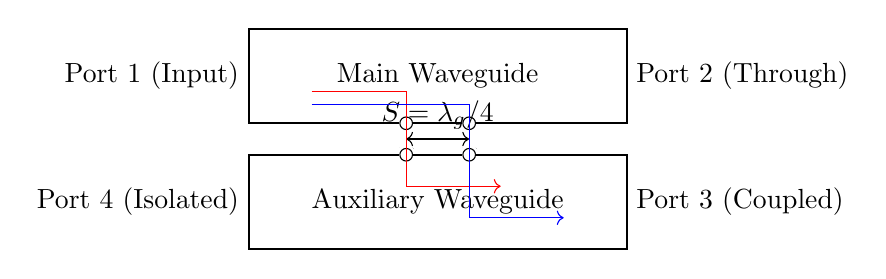
\begin{tikzpicture}[scale=0.8]
    % Main Waveguide
    \draw[thick] (0, 0) rectangle (6, 1.5);
    \node at (3, 0.75) {Main Waveguide};
    \node[left] at (0, 0.75) {Port 1 (Input)};
    \node[right] at (6, 0.75) {Port 2 (Through)};
    
    % Aux Waveguide
    \draw[thick] (0, -2) rectangle (6, -0.5);
    \node at (3, -1.25) {Auxiliary Waveguide};
    \node[left] at (0, -1.25) {Port 4 (Isolated)};
    \node[right] at (6, -1.25) {Port 3 (Coupled)};
    
    % Holes
    \foreach \x in {2.5, 3.5} {
        \draw[dashed, ->] (\x, 0) -- (\x, -0.5);
        \filldraw[white] (\x-0.1, -0.1) rectangle (\x+0.1, 0.1);
        \draw (\x, 0) circle (0.1);
        \filldraw[white] (\x-0.1, -0.6) rectangle (\x+0.1, -0.4);
        \draw (\x, -0.5) circle (0.1);
    }
    \draw[<->] (2.5, -0.25) -- (3.5, -0.25) node[midway, above] {$S = \lambda_g/4$};
   
    % Wave paths
    \draw[->, red] (1, 0.5) -- (2.5, 0.5) -- (2.5, -1) -- (4, -1);
    \draw[->, blue] (1, 0.3) -- (3.5, 0.3) -- (3.5, -1.5) -- (5, -1.5);
\end{tikzpicture}
\end{answerdiagram}

\textbf{Working Principle:}
\begin{itemize}
    \item \keyword{Spacing}: Two holes are spaced apart by distance $S = \lambda_g/4$.
    \item \keyword{Forward Wave}: Signal travels from Port 1. Part of it couples through hole A and hole B towards Port 3. Path difference is zero (waves travel same distance). They add up \keyword{in phase} at Port 3.
    \item \keyword{Reverse Wave}: Waves coupled towards Port 4 have a path difference of $2S = \lambda_g/2$ ($180^\circ$). They \keyword{cancel out} due to destructive interference.
\end{itemize}

\textbf{Parameters:}
\begin{itemize}
    \item Coupling Factor (dB) = $10 \log_{10}(P_1/P_3)$
    \item Directivity (dB) = $10 \log_{10}(P_3/P_4)$
\end{itemize}
\end{solutionbox}

\begin{mnemonicbox}
\mnemonic{Two Holes, Two Directions, Total Control}
\end{mnemonicbox}

\questionmarks{2(c)}{7}{Describe Propagation of microwaves through waveguide and get the equation of cut off wavelength.}

\begin{solutionbox}
\textbf{Wave Propagation:}
Microwaves propagate in waveguides via reflections from conducting walls. They support TE (Transverse Electric) and TM (Transverse Magnetic) modes.

\textbf{Cut-off Wavelength Derivation:}
The wave equation for $H_z$ in a rectangular waveguide (TE mode):
\[ \nabla^2 H_z + \omega^2 \mu \epsilon H_z = 0 \]
Applying boundary conditions for dimensions $a \times b$:
\[ \gamma_{mn}^2 = \left( \frac{m\pi}{a} \right)^2 + \left( \frac{n\pi}{b} \right)^2 - \omega^2 \mu \epsilon \]
For propagation, $\gamma$ must be imaginary (propagation constant $j\beta$). The transition occurs when $\gamma = 0$:
\[ \omega_c^2 \mu \epsilon = \left( \frac{m\pi}{a} \right)^2 + \left( \frac{n\pi}{b} \right)^2 \]
Since $\omega_c = 2\pi f_c$ and $c = 1/\sqrt{\mu\epsilon}$:
\[ \left( \frac{2\pi f_c}{c} \right)^2 = \left( \frac{m\pi}{a} \right)^2 + \left( \frac{n\pi}{b} \right)^2 \]
\[ f_c = \frac{c}{2} \sqrt{\left( \frac{m}{a} \right)^2 + \left( \frac{n}{b} \right)^2} \]
The cut-off wavelength $\lambda_c = c/f_c$:
\[ \lambda_c = \frac{2}{\sqrt{\left( \frac{m}{a} \right)^2 + \left( \frac{n}{b} \right)^2}} \]

\textbf{For Dominant Mode (TE$_{10}$):}
$m=1, n=0$:
\[ \lambda_c = \frac{2}{\sqrt{(1/a)^2}} = 2a \]

\begin{answerdiagram}{Mode Hierarchy}
\begin{tikzpicture}[auto, node distance=1.5cm]
    \node [gtu state] (te10) {TE$_{10}$\\(Dominant)};
    \node [gtu state, right=of te10] (te20) {TE$_{20}$};
    \node [gtu state, below=of te10] (te01) {TE$_{01}$};
    \node [gtu state, right=of te01] (te11) {TE$_{11}$};
    
    \draw [gtu arrow] (te10) -- (te20);
    \draw [gtu arrow] (te10) -- (te01);
    \draw [gtu arrow] (te20) -- (te11);
    \draw [gtu arrow] (te01) -- (te11);
\end{tikzpicture}
\end{answerdiagram}
\end{solutionbox}

\begin{mnemonicbox}
\mnemonic{Cut-off Comes, Propagation Proceeds}
\end{mnemonicbox}

\orquestionmarks{2(a)}{3}{Explain Impedance Matching using Single stub.}

\begin{solutionbox}
\textbf{Single Stub Matching:}
A technique to match a load impedance $Z_L$ to the transmission line characteristic impedance $Z_0$ using a parallel (shunt) stub.

\begin{answerdiagram}{Single Stub Matching}
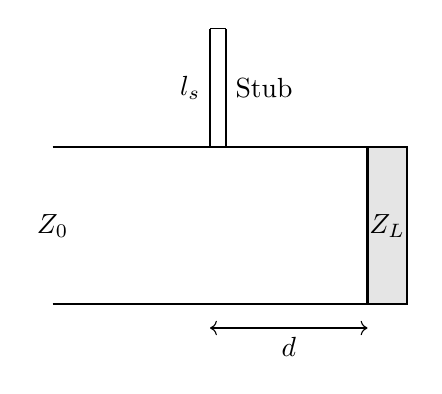
\begin{tikzpicture}[scale=1]
    \draw[thick] (0,2) -- (4,2);
    \draw[thick] (0,0) -- (4,0);
    \draw[thick, fill=gray!20] (4,0) rectangle (4.5,2);
    \node at (4.25,1) {$Z_L$};
    
    \draw[thick] (2,2) -- (2,3.5);
    \draw[thick] (2.2,2) -- (2.2,3.5);
    \draw (2,3.5) -- (2.2,3.5); % Short circuit
    \node[left] at (2, 2.75) {$l_s$};
    \node[right] at (2.2, 2.75) {Stub};
    
    \draw[<->] (2, -0.3) -- (4, -0.3) node[midway, below] {$d$};
    \node at (0,1) {$Z_0$};
\end{tikzpicture}
\end{answerdiagram}

\textbf{Principle:}
\begin{enumerate}
    \item Move from load $Z_L$ distance $d$ towards source until the real part of admittance is matched: $Y_{in} = Y_0 + jB$.
    \item Attach a stub of length $l_s$ at that point with susceptance $-jB$.
    \item Total admittance becomes $Y_{total} = (Y_0 + jB) - jB = Y_0$ (Matched).
\end{enumerate}
\end{solutionbox}

\begin{mnemonicbox}
\mnemonic{Single Stub Solves Susceptance}
\end{mnemonicbox}

\orquestionmarks{2(b)}{4}{Explain Hybrid ring with necessary sketch.}

\begin{solutionbox}
\textbf{Hybrid Ring (Rat-Race Coupler):}
A 4-port directive coupler used for splitting power or combining signals.

\begin{answerdiagram}{Hybrid Ring Structure}
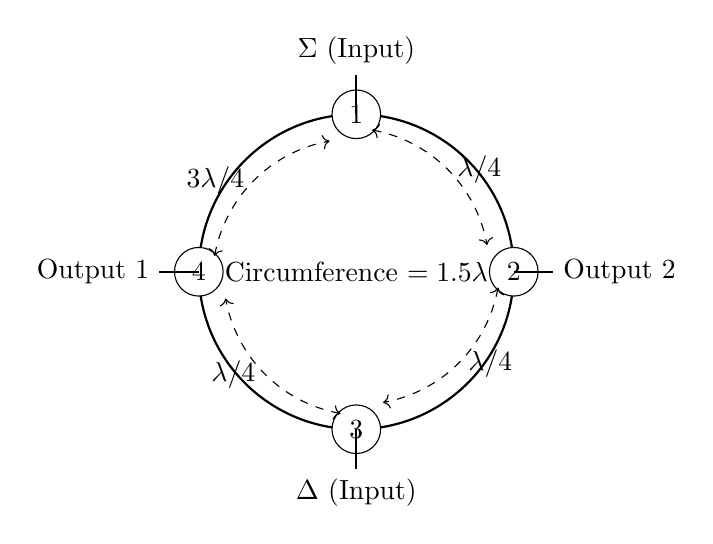
\begin{tikzpicture}
    % Ring
    \draw[thick] (0,0) circle (2);
    
    % Ports
    \node[draw, circle, fill=white] at (0,2) (p1) {1};
    \node[draw, circle, fill=white] at (2,0) (p2) {2};
    \node[draw, circle, fill=white] at (0,-2) (p3) {3};
    \node[draw, circle, fill=white] at (-2,0) (p4) {4};
    
    % Lines connecting ports
    \draw[thick] (0,2) -- (0,2.5) node[above] {$\Sigma$ (Input)};
    \draw[thick] (2,0) -- (2.5,0) node[right] {Output 2};
    \draw[thick] (0,-2) -- (0,-2.5) node[below] {$\Delta$ (Input)};
    \draw[thick] (-2,0) -- (-2.5,0) node[left] {Output 1};
    
    % Distances
    \draw[<->, dashed] (0.2,1.8) arc (80:10:1.8) node[midway, right] {$\lambda/4$};
    \draw[<->, dashed] (1.8,-0.2) arc (-10:-80:1.8) node[midway, right] {$\lambda/4$};
    \draw[<->, dashed] (-0.2,-1.8) arc (-100:-170:1.8) node[midway, left] {$\lambda/4$};
    \draw[<->, dashed] (-1.8,0.2) arc (170:100:1.8) node[midway, left] {$3\lambda/4$};
    
    \node at (0,0) {Circumference $= 1.5\lambda$};
\end{tikzpicture}
\end{answerdiagram}

\textbf{Working:}
\begin{itemize}
    \item Input at Port 1 splits equally to Port 2 and Port 4 (in phase). Port 3 is isolated (path diff $\lambda/2$).
    \item Input at Port 3 splits equally to Port 2 and Port 4 ($180^\circ$ out of phase). Port 1 is isolated.
\end{itemize}
\end{solutionbox}

\begin{mnemonicbox}
\mnemonic{Ring Rotates, Ports Pair-up}
\end{mnemonicbox}

\orquestionmarks{2(c)}{7}{Explain construction, working and any one application of Magic Tee with necessary diagram.}

\begin{solutionbox}
\textbf{Magic Tee (E-H Plane Tee):}
A 4-port hybrid waveguide junction that combines the properties of E-plane and H-plane Tees.

\begin{answerdiagram}{Magic Tee Construction}
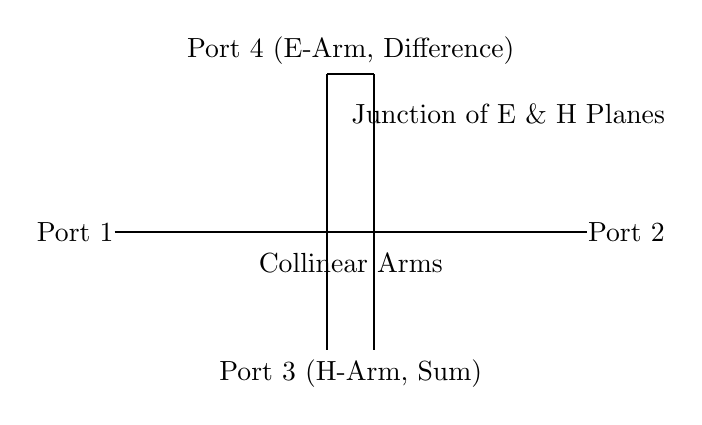
\begin{tikzpicture}[scale=1]
    % Arms
    \draw[thick] (-3,0) -- (3,0); 
    \node at (-3.5,0) {Port 1};
    \node at (3.5,0) {Port 2};
    \node at (0,-0.4) {Collinear Arms};

    % E-Arm
    \draw[thick] (-0.3,0) -- (-0.3,2);
    \draw[thick] (0.3,0) -- (0.3,2);
    \draw[thick] (-0.3,2) -- (0.3,2);
    \node[above] at (0,2) {Port 4 (E-Arm, Difference)};

    % H-Arm
    \draw[thick] (-0.3,0) -- (-0.3,-1.5);
    \draw[thick] (0.3,0) -- (0.3,-1.5);
    \node[below] at (0,-1.5) {Port 3 (H-Arm, Sum)};
    
    \node at (2,1.5) {Junction of E \& H Planes};
\end{tikzpicture}
\end{answerdiagram}

\textbf{Working Principle:}
\begin{itemize}
    \item \keyword{H-Arm Input (Port 3)}: Power splits equally between Port 1 and Port 2 \textbf{in phase}. Port 4 is isolated. ($P_1 = P_2 = P_3/2$).
    \item \keyword{E-Arm Input (Port 4)}: Power splits equally between Port 1 and Port 2 but \textbf{out of phase} ($180^\circ$). Port 3 is isolated.
    \item \keyword{Matched}:Ideally, if ports are matched, $S_{34}=S_{43}=0$ (Isolation).
\end{itemize}

\textbf{Application: Radar Duplexer:}
\begin{itemize}
    \item Transmitter connected to H-Arm (Port 3).
    \item Antenna connected to E-Arm (Port 4).
    \item Receiver connected to one collinear arm, Matched load to other.
    \item Allows single antenna for Tx and Rx by utilizing isolation properties.
\end{itemize}
\end{solutionbox}

\begin{mnemonicbox}
\mnemonic{Magic Makes Isolation, Tee Transmits Together}
\end{mnemonicbox}

\questionmarks{3(a)}{3}{Explain Attenuation measurement with the help of block diagram.}

\begin{solutionbox}
\textbf{Attenuation Measurement:}

\begin{answerdiagram}{Attenuation Measurement Setup}
\begin{tikzpicture}[auto, node distance=1cm]
    \node [gtu start] (gen) {Microwave\\Source};
    \node [gtu block, right=of gen] (iso) {Isolator};
    \node [gtu block, right=of iso] (dut) {Attenuator\\(Variable)};
    \node [gtu stop, right=of dut] (meter) {Power\\Meter};
    
    \draw [gtu arrow] (gen) -- (iso);
    \draw [gtu arrow] (iso) -- (dut);
    \draw [gtu arrow] (dut) -- (meter);
\end{tikzpicture}
\end{answerdiagram}

\textbf{Method:}
\begin{enumerate}
    \item \textbf{Reference}: Measure Power $P_1$ without the device under test (DUT).
    \item \textbf{Measure}: Insert DUT and measure Power $P_2$.
    \item \textbf{Calculate}: Attenuation (dB) $= 10 \log_{10} \frac{P_1}{P_2}$.
\end{enumerate}
\end{solutionbox}

\begin{mnemonicbox}
\mnemonic{Attenuation = Power1 / Power2}
\end{mnemonicbox}

\questionmarks{3(b)}{4}{Explain velocity modulation in two cavity klystron with the help of Applegate diagram.}

\begin{solutionbox}
\textbf{Two Cavity Klystron:}

\begin{answerdiagram}{Klystron Structure}
\begin{tikzpicture}[auto, node distance=1.5cm]
    \node [gtu start] (gun) {Electron\\Gun};
    \node [gtu block, right=of gun] (cav1) {Buncher\\Cavity};
    \node [gtu block, right=of cav1, minimum width=2.5cm] (drift) {Drift Space};
    \node [gtu block, right=of drift] (cav2) {Catcher\\Cavity};
    \node [gtu stop, right=of cav2] (col) {Collector};
    
    \draw [gtu arrow] (gun) -- (cav1);
    \draw [gtu arrow] (cav1) -- (drift);
    \draw [gtu arrow] (drift) -- (cav2);
    \draw [gtu arrow] (cav2) -- (col);
    
    \node [above=of cav1] {RF In};
    \node [above=of cav2] {RF Out};
    \draw [->] (1.5,1) -- (cav1);
    \draw [->] (cav2) -- (6,1);
\end{tikzpicture}
\end{answerdiagram}

\textbf{Velocity Modulation (Applegate Diagram):}

\begin{answerdiagram}{Applegate Diagram}
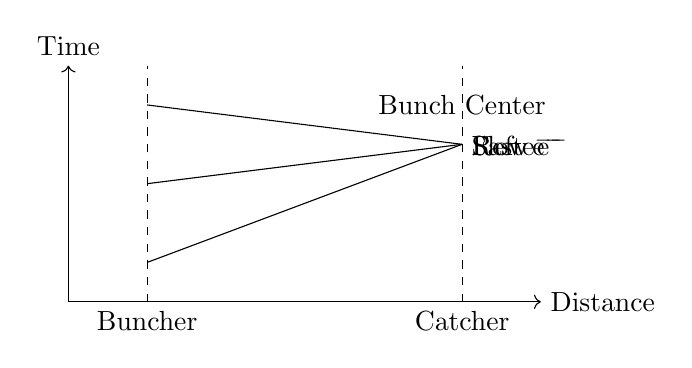
\begin{tikzpicture}
    \draw[->] (0,0) -- (6,0) node[right] {Distance};
    \draw[->] (0,0) -- (0,3) node[above] {Time};
    
    % Buncher Line
    \draw[dashed] (1,0) -- (1,3);
    \node[below] at (1,0) {Buncher};
    
    % Catcher Line
    \draw[dashed] (5,0) -- (5,3);
    \node[below] at (5,0) {Catcher};

    % Electron paths
    \draw (1,0.5) -- (5,2) node[right] {Slow e$^-$}; % Late, Slow
    \draw (1,1.5) -- (5,2) node[right] {Ref e$^-$};  % Mean, Ref
    \draw (1,2.5) -- (5,2) node[right] {Fast e$^-$}; % Early, Fast
    
    \node at (5,2.5) {Bunch Center};
\end{tikzpicture}
\end{answerdiagram}

\textbf{Process:}
\begin{enumerate}
    \item \keyword{Modulation}: RF input voltage at buncher cavity accelerates some electrons (fast) and retards others (slow).
    \item \keyword{Drift}: In the drift space, fast electrons catch up to slow electrons.
    \item \keyword{Bunching}: Electrons group together into bunches, converting continuous beam into pulsed beam containing RF energy.
\end{enumerate}
\end{solutionbox}

\begin{mnemonicbox}
\mnemonic{Velocity Varies, Bunching Builds}
\end{mnemonicbox}

\questionmarks{3(c)}{7}{Explain the principle, construction and effect of electric and magnetic field in Magnetron.}

\begin{solutionbox}
\textbf{Cavity Magnetron:}
A high-power microwave oscillator utilizing \keyword{crossed electric and magnetic fields}.

\begin{answerdiagram}{Magnetron Structure}
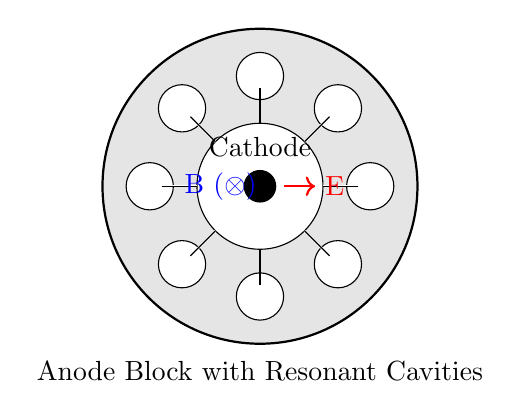
\begin{tikzpicture}
    % Anode Block
    \draw[thick, fill=gray!20] (0,0) circle (2);
    \draw[fill=white] (0,0) circle (0.8);
    
    % Cavities
    \foreach \a in {0,45,...,315} {
        \draw[fill=white] (\a:1.4) circle (0.3);
        \draw[white, thick] (\a:1.4) -- (\a:0.8); % Open to interaction space
        \draw (\a:1.25) -- (\a:0.8);
    }
    
    % Cathode
    \draw[fill=black] (0,0) circle (0.2);
    \node at (0,0.5) {Cathode};
    
    % Fields
    \draw[->, red, thick] (0.3,0) -- (0.7,0) node[right] {E};
    \node[blue] at (-0.5,0) {B ($\otimes$)};
    
    \node[below] at (0,-2.1) {Anode Block with Resonant Cavities};
\end{tikzpicture}
\end{answerdiagram}

\textbf{Effect of Fields:}
\begin{itemize}
    \item \keyword{Electric Field (E)}: Radial, from anode (+) to cathode (-). Accelerates electrons outward.
    \item \keyword{Magnetic Field (B)}: Axial (perpendicular to page). Exerts Lorentz force $F = q(v \times B)$, bending electron path.
\end{itemize}

\textbf{Electron Motion:}
\begin{enumerate}
    \item \textbf{Low B}: Electrons go straight to anode.
    \item \textbf{Critical B ($B_c$)}: Electrons graze anode.
    \item \textbf{Operating B ($>B_c$)}: Electrons spiral in interactions space, forming "spokes", transferring energy to RF fields in cavities before returning to cathode or being collected.
\end{enumerate}
\end{solutionbox}

\begin{mnemonicbox}
\mnemonic{Magnetron Makes Microwaves via Magnetic Motion}
\end{mnemonicbox}

\orquestionmarks{3(a)}{3}{Explain working of TWT (Travelling Wave Tube) as an Amplifier.}

\begin{solutionbox}
\textbf{Travelling Wave Tube (TWT):}
A broadband microwave amplifier utilizing a \keyword{Slow Wave Structure} (Helix).

\begin{answerdiagram}{TWT Schematic}
\begin{tikzpicture}[auto, node distance=1.5cm]
    \node [gtu start] (gun) {Gun};
    \node [gtu block, right=of gun, minimum width=4cm] (helix) {Helix (Slow Wave)};
    \node [gtu stop, right=of helix] (col) {Collector};
    
    \draw [gtu arrow] (gun) -- (helix);
    \draw [gtu arrow] (helix) -- (col);
    
    \draw [<-] (2, 0.5) -- (2, 1) node[above] {RF In};
    \draw [->] (5, 0.5) -- (5, 1) node[above] {RF Out};
    
    \node [below] at (3.5, -0.5) {Electron Beam};
\end{tikzpicture}
\end{answerdiagram}

\textbf{Working:}
\begin{itemize}
    \item \keyword{Slow Wave}: The helix reduces the RF wave velocity ($v_p$) to match electron beam velocity ($v_e$).
    \item \keyword{Interaction}: Continuous interaction occurs along the tube. Electrons are bunched by the RF field and transfer kinetic energy to the RF wave, amplifying it.
\end{itemize}
\end{solutionbox}

\begin{mnemonicbox}
\mnemonic{Travelling Wave Transfers Energy}
\end{mnemonicbox}

\orquestionmarks{3(b)}{4}{Explain Bolometer method for low power measurement at microwave frequency.}

\begin{solutionbox}
\textbf{Bolometer Method:}
Uses a temperature-sensitive resistive element (Barretter or Thermistor) in a bridge circuit.

\begin{answerdiagram}{Bolometer Bridge Circuit}
\begin{circuitikz}[scale=1]
    \draw (0,0) to[R, l=$R_1$] (0,2) -- (2,2) to[R, l=$R_{Bolometer}$] (2,0) -- (0,0);
    \draw (0,2) -- (-1,2) to[V, l=$V_{DC}$] (-1,0) -- (0,0);
    \draw (0,2) -- (0,3) to[short] (2,3) -- (2,2); % Measurement tap
    \node at (1, 2.5) {To Detector/Amp};
    \node at (1,1) {Bridge};
    \draw [->] (3,1) -- (2.5,1) node[right] {$\mu$Wave Power};
\end{circuitikz}
\end{answerdiagram}

\textbf{Working:}
\begin{enumerate}
    \item Bridge is initially balanced with DC Power.
    \item Microwave power heats the element $\to$ Resistance changes $\to$ Bridge unbalance.
    \item Amount of unbalance or change in DC bias required to re-balance is proportional to RF power.
\end{enumerate}
\end{solutionbox}

\begin{mnemonicbox}
\mnemonic{Bolometer Burns, Bridge Balances}
\end{mnemonicbox}

\orquestionmarks{3(c)}{7}{Explain frequency and wavelength measurement method with the help of block diagram.}

\begin{solutionbox}
\textbf{Frequency Measurement (Heterodyne Method):}

\begin{answerdiagram}{Heterodyne Frequency Meter}
\begin{tikzpicture}[auto, node distance=1.5cm]
    \node [gtu input] (rf) {Unknown RF};
    \node [gtu block, right=of rf] (mixer) {Mixer};
    \node [gtu block, above=of mixer] (lo) {Local Osc};
    \node [gtu block, right=of mixer] (filter) {Low Pass Filter};
    \node [gtu stop, right=of filter] (counter) {Counter};
    
    \draw [gtu arrow] (rf) -- (mixer);
    \draw [gtu arrow] (lo) -- (mixer);
    \draw [gtu arrow] (mixer) -- (filter);
    \draw [gtu arrow] (filter) -- (counter);
\end{tikzpicture}
\end{answerdiagram}

\textbf{Wavelength Measurement (Slotted Line Method):}

\begin{answerdiagram}{Slotted Line Setup}
\begin{tikzpicture}[auto, node distance=1cm]
    \node [gtu start] (src) {Source};
    \node [gtu block, right=of src] (iso) {Isolator};
    \node [gtu block, right=of iso, minimum width=3cm] (slot) {Slotted Line};
    \node [gtu stop, right=of slot] (load) {Short/Load};
    
    \draw [gtu arrow] (src) -- (iso);
    \draw [gtu arrow] (iso) -- (slot);
    \draw [gtu arrow] (slot) -- (load);
    
    \node [above=0.2cm of slot] (probe) {Movable Probe};
    \draw [->] (probe) -- (slot);
\end{tikzpicture}
\end{answerdiagram}

\textbf{Procedure:}
\begin{enumerate}
    \item \textbf{Measure}: Locate two adjacent minima (nodes) on the slotted line. Let locations be $d_1$ and $d_2$.
    \item \textbf{Calculate $\lambda_g$}: Distance between minima is $\lambda_g/2$.
    \[ \lambda_g = 2 |d_1 - d_2| \]
    \item \textbf{Calculate Frequency}:
    \[ \frac{1}{\lambda_0^2} = \frac{1}{\lambda_g^2} + \frac{1}{\lambda_c^2} \quad \text{and} \quad f = \frac{c}{\lambda_0} \]
\end{enumerate}
\end{solutionbox}

\begin{mnemonicbox}
\mnemonic{Frequency First, Wavelength With-measurement}
\end{mnemonicbox}

% End of Part 1 content

\questionmarks{4(a)}{3}{State Frequency limitations of vacuum tubes at microwave frequency.}

\begin{solutionbox}
\textbf{Frequency Limitations:}

\begin{itemize}
    \item \textbf{Transit time effects}: Electron transit time becomes comparable to RF period, causing phase delay and reducing efficiency.
    \item \textbf{Inter-electrode capacitance}: Reactance ($X_c = 1/2\pi fC$) decreases, shunting the output and reducing gain.
    \item \textbf{Lead inductance}: Parasitic inductance of connecting leads causes resonance and instability.
    \item \textbf{Skin effect}: Current flows only on surface, increasing effective resistance and losses.
\end{itemize}

\textbf{Limiting Factors Table:}
\begin{tabulary}{\linewidth}{|L|L|}
\hline
\textbf{Factor} & \textbf{Effect} \\ \hline
Transit Time & Phase delay ($f < 1/2\pi\tau$) \\ \hline
Capacitance & Gain drop ($\propto 1/f$) \\ \hline
Lead Inductance & Resonance/Instability \\ \hline
Skin Effect & Increased Resistance \\ \hline
\end{tabulary}
\end{solutionbox}

\begin{mnemonicbox}
\mnemonic{Transit Time Troubles Traditional Tubes}
\end{mnemonicbox}

\questionmarks{4(b)}{4}{Explain working of IMPATT diode with proper sketch.}

\begin{solutionbox}
\textbf{IMPATT Diode (Impact Ionization Avalanche Transit Time):}

\begin{answerdiagram}{IMPATT Diode Structure}
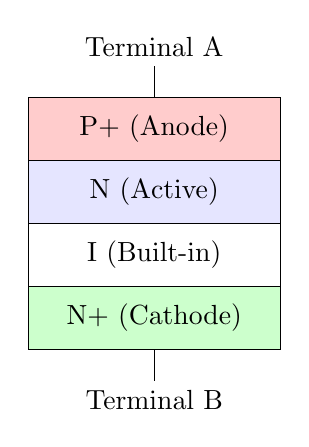
\begin{tikzpicture}[scale=0.8]
    % Layers
    \draw[fill=red!20] (0,3) rectangle (4,4) node[midway] {P+ (Anode)};
    \draw[fill=blue!10] (0,2) rectangle (4,3) node[midway] {N (Active)};
    \draw[fill=white] (0,1) rectangle (4,2) node[midway] {I (Built-in)};
    \draw[fill=green!20] (0,0) rectangle (4,1) node[midway] {N+ (Cathode)};
    
    % Terminals
    \draw (2,4) -- (2,4.5) node[above] {Terminal A};
    \draw (2,0) -- (2,-0.5) node[below] {Terminal B};
\end{tikzpicture}
\end{answerdiagram}

\textbf{Working Principle:}
Generates negative resistance using two effects:
\begin{enumerate}
    \item \textbf{Impact Ionization (Avalanche Effect)}: Creates a phase delay of $90^\circ$ between voltage and current.
    \item \textbf{Transit Time Effect}: Carriers drifting through the drift region create another $90^\circ$ delay.
\end{enumerate}
\textbf{Total Delay}: $180^\circ$ phase shift $\rightarrow$ Negative Resistance (Current opposes voltage).

\begin{answerdiagram}{Negative Resistance Cycle}
\begin{tikzpicture}[auto, node distance=1.5cm]
    \node [gtu state] (high) {High Field};
    \node [gtu state, right=of high] (avalanche) {Avalanche\\Breakdown};
    \node [gtu state, below=of avalanche] (carriers) {Carrier\\Generation};
    \node [gtu state, left=of carriers] (transit) {Transit\\Delay};
    \node [gtu state, above=of transit] (peak) {Current Peak\\($180^\circ$ lag)};
    
    \draw [gtu arrow] (high) -- (avalanche);
    \draw [gtu arrow] (avalanche) -- (carriers);
    \draw [gtu arrow] (carriers) -- (transit);
    \draw [gtu arrow] (transit) -- (peak);
    \draw [gtu arrow] (peak) -- (high);
\end{tikzpicture}
\end{answerdiagram}
\end{solutionbox}

\begin{mnemonicbox}
\mnemonic{Impact Ionization, Transit Time = Negative Resistance}
\end{mnemonicbox}

\questionmarks{4(c)}{7}{Explain Principle, tunneling phenomenon and any one application of Tunnel Diode.}

\begin{solutionbox}
\textbf{Tunnel Diode Principle:}
Operates on the \keyword{Quantum Mechanical Tunneling} effect across a thin potential barrier in a heavily doped p-n junction ($10^{19}$ to $10^{20}$ doping).

\textbf{Energy Band Diagram:}

\begin{answerdiagram}{Tunnel Diode Band Diagram (Peak Point)}
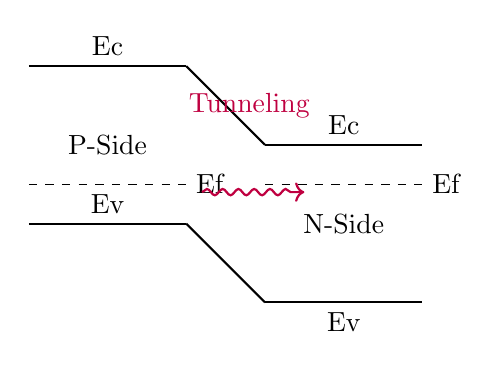
\begin{tikzpicture}
    % P-side
    \draw[thick] (0,0) -- (2,0) node[midway, above] {Ev};
    \draw[thick] (0,2) -- (2,2) node[midway, above] {Ec};
    \draw[dashed] (0,0.5) -- (2,0.5) node[right] {Ef};
    \node at (1,1) {P-Side};
    
    % Barrier
    \draw[thick] (2,0) -- (3, -1);
    \draw[thick] (2,2) -- (3, 1);
    
    % N-side
    \draw[thick] (3,-1) -- (5,-1) node[midway, below] {Ev};
    \draw[thick] (3,1) -- (5,1) node[midway, above] {Ec};
    \draw[dashed] (3,0.5) -- (5,0.5) node[right] {Ef}; 
    \node at (4,0) {N-Side};
    
    \draw[->, purple, thick, decorate, decoration={snake, amplitude=0.4mm, segment length=2mm, post length=1mm}] (2.2, 0.4) -- (3.5, 0.4); 
    \node[purple] at (2.8, 1.5) {Tunneling};
\end{tikzpicture}
\end{answerdiagram}

\textbf{I-V Characteristics:}

\begin{answerdiagram}{Tunnel Diode I-V Curve}
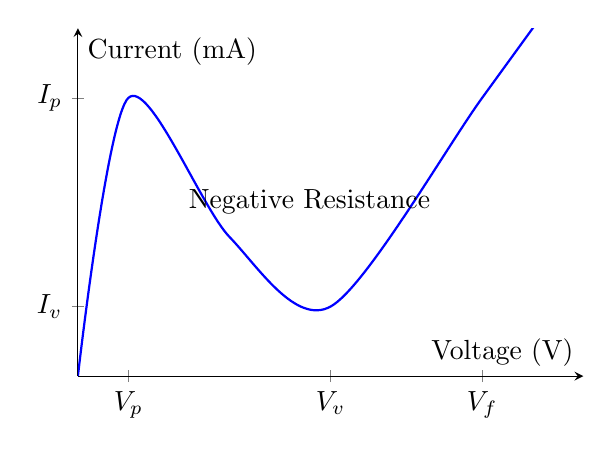
\begin{tikzpicture}
    \begin{axis}[
        xlabel={Voltage (V)},
        ylabel={Current (mA)},
        axis lines=middle,
        xmin=0, xmax=1,
        ymin=0, ymax=10,
        xtick={0.1, 0.5, 0.8},
        xticklabels={$V_p$, $V_v$, $V_f$},
        ytick={2, 8},
        yticklabels={$I_v$, $I_p$},
        width=8cm, height=6cm
    ]
    \addplot[smooth, thick, blue] coordinates {
        (0,0) (0.1,8) (0.3,4) (0.5,2) (0.8,8) (1,12)
    };
    \node[anchor=west] at (axis cs:0.2, 5) {Negative Resistance};
    \end{axis}
\end{tikzpicture}
\end{answerdiagram}

\textbf{Application - Oscillator:}
Operates in the negative resistance region to generate oscillations.
\end{solutionbox}

\begin{mnemonicbox}
\mnemonic{Tunnel Through, Negative Grows, Oscillator Flows}
\end{mnemonicbox}

\orquestionmarks{4(a)}{3}{Explain Hazards due to microwave radiation.}

\begin{solutionbox}
\textbf{Microwave Hazards:}

\begin{enumerate}
    \item \textbf{HERP (Health Hazards to Personnel):}
    \begin{itemize}
        \item \keyword{Thermal}: Tissue heating, cataracts.
        \item \keyword{Non-thermal}: Cellular damage.
    \end{itemize}
    \item \textbf{HERO (Hazards to Ordnance):}
    \begin{itemize}
        \item Premature ignition of explosives.
    \end{itemize}
    \item \textbf{HERF (Hazards to Fuel):}
    \begin{itemize}
        \item Ignition of fuel vapors.
    \end{itemize}
\end{enumerate}

\textbf{Safety Limit:} Generally $< 10 \text{ mW/cm}^2$.
\end{solutionbox}

\begin{mnemonicbox}
\mnemonic{HERP-HERO-HERF = Health-Explosive-Fuel Risks}
\end{mnemonicbox}

\orquestionmarks{4(b)}{4}{Explain Degenerate and non-degenerate mode in Parametric Amplifier.}

\begin{solutionbox}
\textbf{Parametric Amplifier Modes:}

\begin{enumerate}
    \item \textbf{Non-Degenerate Mode:}
    \begin{itemize}
        \item \textbf{Frequencies}: Pump ($f_p$) $\neq$ 2 $\times$ Signal ($f_s$). ($f_p = f_s + f_i$).
        \item \keyword{Idler}: A separate idler frequency $f_i$ exists.
        \item \textbf{Performance}: Better noise figure, stable gain.
    \end{itemize}
    \item \textbf{Degenerate Mode:}
    \begin{itemize}
        \item \textbf{Frequencies}: Pump ($f_p$) = 2 $\times$ Signal ($f_s$).
        \item \keyword{Idler}: Idler equals signal frequency ($f_i = f_s$).
        \item \textbf{Performance}: Output depends on phase of pump.
    \end{itemize}
\end{enumerate}
\end{solutionbox}

\begin{mnemonicbox}
\mnemonic{Non-degenerate = Not-single, Degenerate = Doubled-frequency}
\end{mnemonicbox}

\orquestionmarks{4(c)}{7}{Explain principle and Gunn effect in Gunn Diode. Also Explain Gunn Diode as an Oscillator.}

\begin{solutionbox}
\textbf{Gunn Effect Principle:}
Based on the \keyword{Transferred Electron Effect}. Electrons transfer from high-mobility central valley ($\Gamma$) to low-mobility satellite valley (L).

\begin{answerdiagram}{Gunn Effect Band Structure}
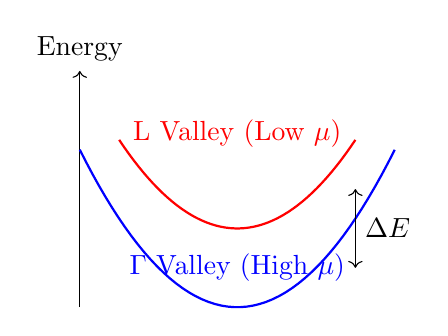
\begin{tikzpicture}
    \draw[->] (0,0) -- (0,3) node[above] {Energy};
    
    % Central Valley
    \draw[thick, blue] plot[domain=0:4, samples=50, variable=\x] ({\x}, {0.5*(\x-2)^2});
    \node[blue] at (2,0.5) {$\Gamma$ Valley (High $\mu$)};
    
    % Satellite Valley
    \draw[thick, red] plot[domain=0.5:3.5, samples=50, variable=\x] ({\x}, {1 + 0.5*(\x-2)^2}); 
    \node[red] at (2,2.2) {L Valley (Low $\mu$)};
    
    \draw[<->] (3.5,0.5) -- (3.5,1.5) node[midway, right] {$\Delta E$};
\end{tikzpicture}
\end{answerdiagram}

\textbf{Gunn Oscillator:}
\begin{itemize}
    \item Gunn diode in resonant cavity.
    \item Frequency $f = v_{domain} / L_{eff}$.
\end{itemize}
\end{solutionbox}

\begin{mnemonicbox}
\mnemonic{Gunn Gets Going via Gallium-Arsenide}
\end{mnemonicbox}

\questionmarks{5(a)}{3}{Explain working principle of Basic RADAR system with the help of block diagram.}

\begin{solutionbox}
\textbf{RADAR Principle:}
Radio Detection And Ranging. Range $R = (c \times t)/2$.

\begin{answerdiagram}{Basic Radar Block Diagram}
\begin{tikzpicture}[auto, node distance=1.5cm]
    \node [gtu block] (tim) {Timer};
    \node [gtu block, below=of tim] (mod) {Modulator};
    \node [gtu block, right=of mod] (tx) {Transmitter};
    \node [gtu block, right=of tx] (dup) {Duplexer};
    \node [gtu block, right=of dup] (ant) {Antenna};
    \node [gtu block, below=of dup] (rx) {Receiver};
    \node [gtu block, left=of rx] (disp) {Display};
    
    \draw [gtu arrow] (tim) -- (mod);
    \draw [gtu arrow] (mod) -- (tx);
    \draw [gtu arrow] (tx) -- (dup);
    \draw [gtu arrow] (dup) -- (ant);
    \draw [gtu arrow] (ant) -- (dup);
    \draw [gtu arrow] (dup) -- (rx);
    \draw [gtu arrow] (rx) -- (disp);
    \draw [gtu arrow] (tim) -| (disp);
\end{tikzpicture}
\end{answerdiagram}
\end{solutionbox}

\begin{mnemonicbox}
\mnemonic{RADAR Ranges by Round-trip Reflection}
\end{mnemonicbox}

\questionmarks{5(b)}{4}{Explain A-scope display method with the help of proper figure.}

\begin{solutionbox}
\textbf{A-Scope Display:}
Displays Amplitude vs Time/Range.

\begin{answerdiagram}{A-Scope Presentation}
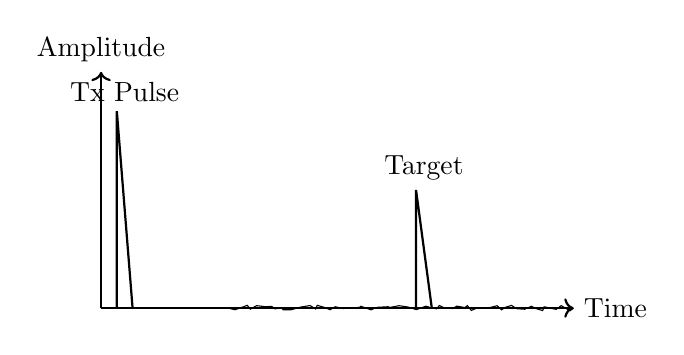
\begin{tikzpicture}
    \draw[->, thick] (0,0) -- (6,0) node[right] {Time};
    \draw[->, thick] (0,0) -- (0,3) node[above] {Amplitude};
    
    \draw[thick] (0.2,0) -- (0.2,2.5) -- (0.4,0); 
    \node[above] at (0.3,2.5) {Tx Pulse};
    
    \draw[thick] (4,0) -- (4,1.5) -- (4.2,0); 
    \node[above] at (4.1,1.5) {Target};
    
    \draw[decorate, decoration={random steps, segment length=2pt, amplitude=1pt}] (1.5,0) -- (6,0); 
\end{tikzpicture}
\end{answerdiagram}
\end{solutionbox}

\begin{mnemonicbox}
\mnemonic{A-scope shows Amplitude Along time Axis}
\end{mnemonicbox}

\questionmarks{5(c)}{7}{Explain Doppler effect and working of MTI (Moving Target Indicator) RADAR system with the help of block diagram.}

\begin{solutionbox}
\textbf{Doppler Effect:} $f_d = 2v_r/\lambda$.

\textbf{MTI Radar:} Uses Doppler to distinguish moving targets.

\begin{answerdiagram}{MTI Radar Block Diagram}
\begin{tikzpicture}[scale=0.8, transform shape, node distance=1.5cm]
    \node [gtu block] (stalo) {STALO};
    \node [gtu block, below=of stalo] (coho) {COHO};
    \node [gtu block, right=of stalo] (mix1) {Mixer 1};
    
    \node [gtu block, above=of mix1] (tx) {Tx};
    \node [gtu block, above=of tx] (ant) {Ant};
    \node [gtu block, right=of mix1] (phase) {Phase Detector};
    \node [gtu block, right=of phase] (delay) {Delay Line ($T_r$)};
    \node [gtu block, right=of delay] (sub) {Subtractor};
    \node [gtu output, right=of sub] (disp) {Display};
    
    \draw [gtu arrow] (stalo) -- (mix1);
    \draw [gtu arrow] (coho) -- (phase);
    \draw [gtu arrow] (mix1) -- (phase);
    \draw [gtu arrow] (phase) -- (delay);
    \draw [gtu arrow] (phase) to[bend left] (sub);
    \draw [gtu arrow] (delay) -- (sub);
    \draw [gtu arrow] (sub) -- (disp);
\end{tikzpicture}
\end{answerdiagram}
\end{solutionbox}

\begin{mnemonicbox}
\mnemonic{MTI Makes Targets Identifiable via Doppler Difference}
\end{mnemonicbox}

\orquestionmarks{5(a)}{3}{Define: a) Blind speed, and b) MUR}

\begin{solutionbox}
\textbf{Definitions:}
\begin{itemize}
    \item \textbf{Blind Speed ($v_b$)}: Target speed where Doppler shift is multiple of PRF. $v_b = \frac{n \lambda f_r}{2}$.
    \item \textbf{MUR}: Maximum Unambiguous Range. $R_{max} = \frac{c}{2 f_r}$.
\end{itemize}
\end{solutionbox}

\begin{mnemonicbox}
\mnemonic{Blind speed Blocks, MUR Measures maximum}
\end{mnemonicbox}

\orquestionmarks{5(b)}{4}{Explain the factors affecting Maximum RADAR range.}

\begin{solutionbox}
\textbf{Radar Range Equation:}
\[ R_{max} = \left[ \frac{P_t G^2 \lambda^2 \sigma}{(4\pi)^3 S_{min}} \right]^{1/4} \]

\textbf{Factors:}
\begin{itemize}
    \item $P_t$: Transmitter Power ($R \propto P_t^{1/4}$).
    \item $G$: Antenna Gain ($R \propto \sqrt{G}$).
    \item $\lambda$: Wavelength ($R \propto \sqrt{\lambda}$).
    \item $\sigma$: Target Cross Section.
    \item $S_{min}$: Receiver Sensitivity.
\end{itemize}
\end{solutionbox}

\begin{mnemonicbox}
\mnemonic{Power-Gain-Lambda-Sigma determine Range}
\end{mnemonicbox}

\orquestionmarks{5(c)}{7}{Compare Pulsed RADAR and CW Doppler RADAR.}

\begin{solutionbox}
\textbf{Comparison:}
\begin{tabulary}{\linewidth}{|L|L|L|}
\hline
\textbf{Parameter} & \textbf{Pulsed} & \textbf{CW Doppler} \\ \hline
Transmission & Pulses & Continuous \\ \hline
Range & Measurable & Not measurable (normally) \\ \hline
Velocity & Difficult & Easy (Doppler) \\ \hline
\end{tabulary}
\end{solutionbox}

\begin{mnemonicbox}
\mnemonic{Pulsed Position gives, CW Continuously Waves}
\end{mnemonicbox}

\end{document}
